\subsection{Use cases} \label{ssc:usecases}
The following use cases have been derived from the understanding of the problem domain and actors described in \autoref{ssc:actors}. The following description of the use cases include how the interactions with the system will take place, which actors are involved, and which functions are called within the system to complete the actions. \\

\fancyLayout{use_case}{Add an asset}
    {Use case for adding an asset}
    {use_case:add_an_asset}
    {
        \textbf{Use Case:} Adding an asset is done by an admin. The admin goes to the add asset page, and fills in the relevant information about the asset. The admin then saves the asset in the system and it becomes visible to all employees.
    
        \vskip 0.2cm
        
        \textbf{Objects:} Admin, Asset
        
        \vskip 0.2cm
        
        \textbf{Functions:} Add asset
    }

\begin{figure}[H]
    \centering
    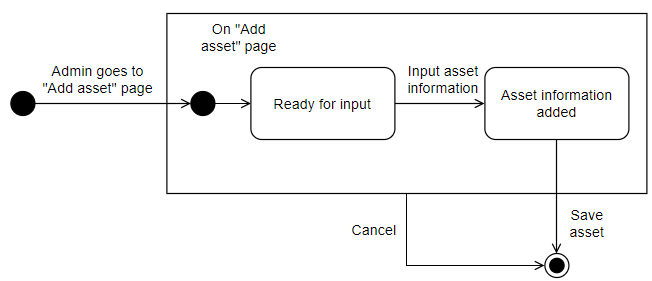
\includegraphics[width=0.80\textwidth]{figures/UseCases/AddAssetUseCase.png}
    \caption{User interface state chart diagram for adding an asset}
    \label{fig:add_asset_statechart}
\end{figure}

%\newpage

\fancyLayout{use_case}{Loan out an asset}
    {Use case for loaning out an asset}
    {use_case:loan_out_an_asset}
    {
        \textbf{Use Case:} Loaning out an asset is done by an admin, whom an employee contacts, when they want to borrow the given asset. The admin goes to the page of the given asset and creates a \textit{Loan} relation. The admin then hands over the asset to the employee.
    
        \vskip 0.2cm
        
        \textbf{Objects:} Admin, Asset, Employee, Loan
        
        \vskip 0.2cm
        
        \textbf{Functions:} Asset loaned out
    }
 
\begin{figure}[H]
    \centering
    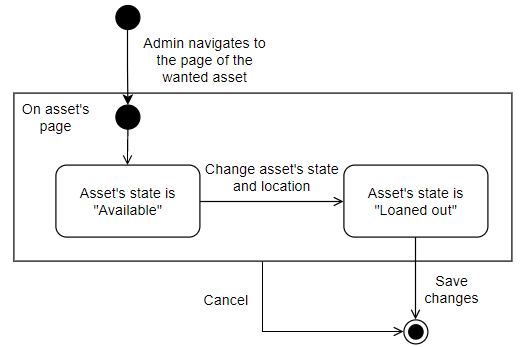
\includegraphics[width=0.75\textwidth]{figures/UseCases/LoanOutAssetUseCase.png}
    \caption{User interface state chart diagram for loaning out an asset}
    \label{fig:loan_out_asse_statechart}
\end{figure}

\newpage
 
\fancyLayout{use_case}{Return an asset}
    {Use case for returning an asset}
    {use_case:return_an_asset}
    {
        \textbf{Use Case:} When an asset is being returned by an employee, it is handed over to an admin. The admin then goes to the page of the given asset and disconnects the \textit{Loan} from the asset.
    
        \vskip 0.2cm
        
        \textbf{Objects:} Admin, Asset, Employee, Loan
        
        \vskip 0.2cm
        
        \textbf{Functions:} Update asset information.
    }
    
\begin{figure}[H]
    \centering
    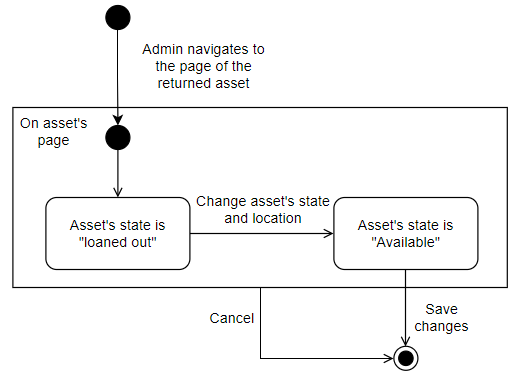
\includegraphics[width=0.75\textwidth]{figures/UseCases/ReturnAssetUseCase.png}
    \caption{User interface state chart diagram for returning an asset}
    \label{fig:return_asset_statechart}
\end{figure}

\fancyLayout{use_case}{Change the information of an asset}
    {Use case for changing the information of an asset}
    {use_case:changing_the_information_about_an_asset}
    {
        \textbf{Use Case:} If one of the properties of an asset changes, the changed data should be updated in the system by an admin. These changes could be the asset going from working to being broken or being updated to a new operation system. To update the asset's information, the admin goes to the given asset's page, then presses the edit button, and changes the outdated data to comply with the new state of the asset in the problem domain.
    
        \vskip 0.2cm
        
        \textbf{Objects:} Admin, Asset
        
        \vskip 0.2cm
        
        \textbf{Functions:} Search for asset, Update asset information, View asset
    }
    
\begin{figure}[H]
    \centering
    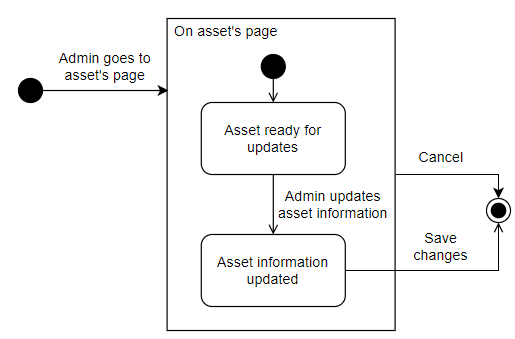
\includegraphics[width=0.75\textwidth]{figures/UseCases/UpdateAssetUseCase.png}
    \caption{User interface state chart diagram for changing an asset}
    \label{fig:edit_asset_statechart}
\end{figure}

\newpage

\fancyLayout{use_case}{Remove an asset}
    {Use case for removing an asset}
    {use_case:remove_an_asset}
    {
        \textbf{Use Case:} When an asset is no longer needed within the problem domain, it is discarded. This is handled in the system by an admin. The admin goes to the page of the given asset and deletes it from the system.
        \vskip 0.2cm
        
        \textbf{Objects:} Admin, Asset
        
        \vskip 0.2cm
        
        \textbf{Functions:} Remove asset
    }

\begin{figure}[H]
    \centering
    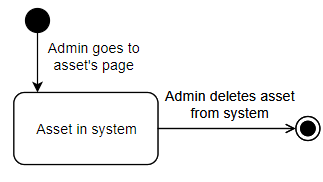
\includegraphics[width=0.5\textwidth]{figures/UseCases/DeleteAssetUseCase.png}
    \caption{User interface state chart diagram for removing an asset}
    \label{fig:remove_asset_statechart}
\end{figure}

\newpage

\fancyLayout{use_case}{Search for an asset}
    {Use case for searching for an asset}
    {use_case:search_for_an_asset}
    {
        \textbf{Use Case:} If a user wants information about a specific asset, this can be achieved by going to the search page and entering some information about the asset in the search field. The system then returns a list of assets complying with the search query. The user can then choose the desired asset to manage.
    
        \vskip 0.2cm
        
        \textbf{Objects:} Admin, Asset, Employee
        
        \vskip 0.2cm
        
        \textbf{Functions:} Search for asset
    }

\begin{figure}[H]
    \centering
    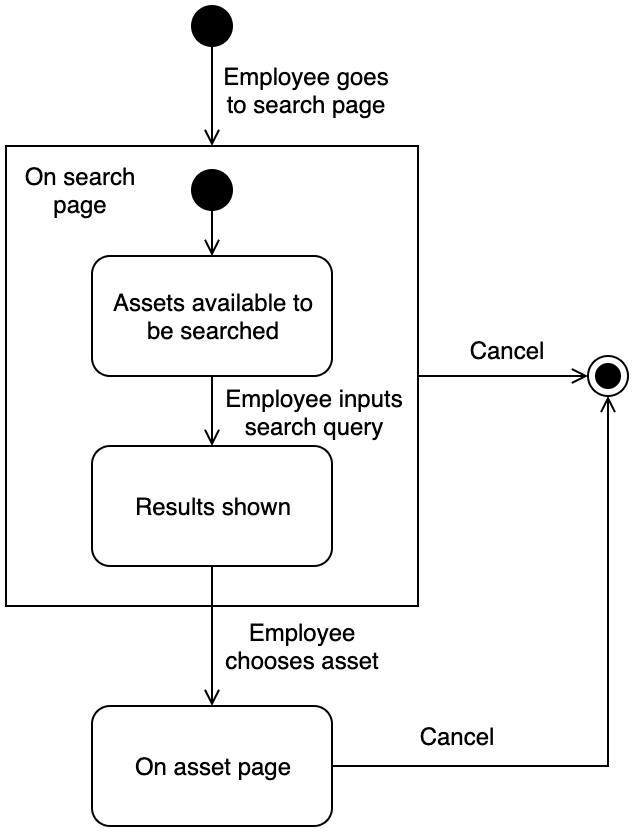
\includegraphics[width=0.5\textwidth]{figures/UseCases/UC_Search_asset.png}
    \caption{User interface state chart diagram for searching for an asset}
    \label{fig:search_asset_statechart}
\end{figure}

\fancyLayout{use_case}{Comment on an asset}
    {Use case for commenting on an asset}
    {use_case:commenting_on_an_asset}
    {
        \textbf{Use Case:} A user might have a comment regarding an asset, such as an issue they have had with it or suggestions for improvements. To share this information with other users, they can go to the page of the asset and add a comment to it. This comment will be visible to all users.
    
        \vskip 0.2cm
        
        \textbf{Objects:} Admin, Asset, Employee
        
        \vskip 0.2cm
        
        \textbf{Functions:} Add comment to asset, Search for asset, View Asset
    }

\begin{figure}[H]
    \centering
    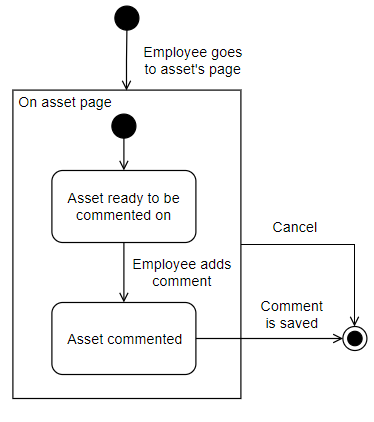
\includegraphics[width=0.5\textwidth]{figures/UseCases/CommentAssetUseCase.png}
    \caption{User interface state chart diagram for adding a comment to an asset}
    \label{fig:add_comment_statechart}
\end{figure}

In addition to the already described interactions stated in the system definition, the interviews with Aalborg Zoo have let to the use case of an admin exporting a list of assets from the system. The report can consist of all or some of the assets in the system and will be saved as a file on the admins computer.

\fancyLayout{use_case}{Print a list of assets}
    {Use case for printing a list of assets}
    {use_case:print_a_report_of_assets}
    {
        \textbf{Use Case:} As the number of assets in the system increases, an admin might want to retrieve a smaller number of assets from the system. The admin goes to the page containing the list of assets, selects the assets they want to retrieve from the system and presses the export button. The system then generates a file containing information about the selected assets and saves it on the admin's computer.
    
        \vskip 0.2cm
        
        \textbf{Objects:} Admin, Asset
        
        \vskip 0.2cm
        
        \textbf{Functions:} Export list of assets
    }

\begin{figure}[H]
    \centering
    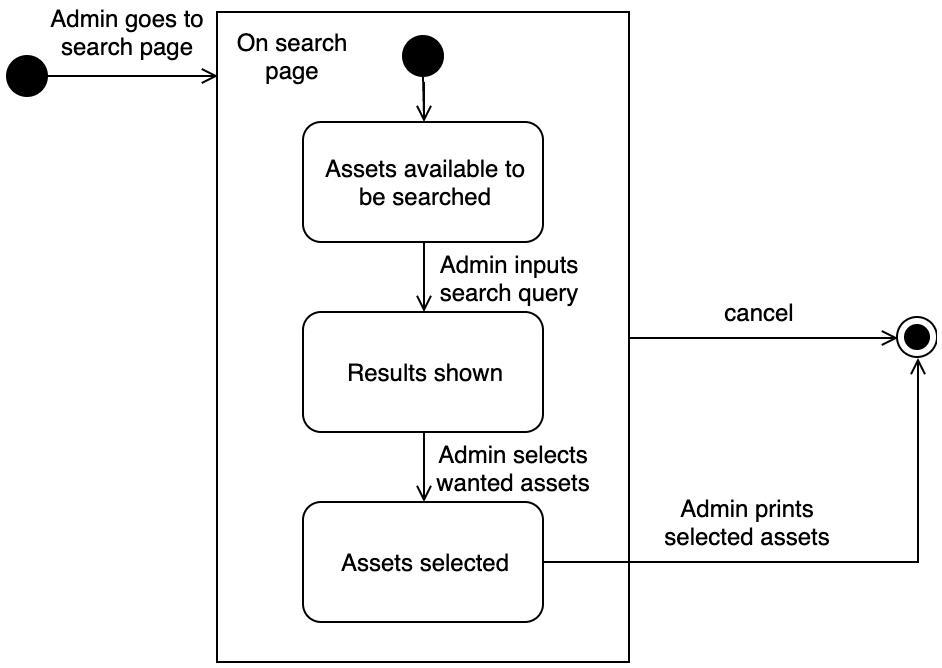
\includegraphics[width=0.70\textwidth]{figures/UseCases/UC_Print_report.png}
    \caption{User interface state chart diagram for printing out a report}
    \label{fig:print_report_statechart}
\end{figure}

These are the relevant use cases for managing the assets. The use cases have been placed in an actor table (see \autoref{tab:actor_table}) with the two previously described actors in order to illustrate the connections between these.

\begin{table}[H]
    \centering
    % \hrule
    \vspace{0.2cm}
    \hspace{6cm} \vspace{0.6cm} \textbf{Actors}
    \begin{tabular}{p{0.5\textwidth} || p{0.2\textwidth} p{0.2\textwidth}}
        \textbf{Use cases} & Admin & Employee \vspace{0.2cm}\\
        \hline \hline
        Add an asset & \hspace{0.34cm} \checkmark & \\
        \hline
        Loan out an asset & \hspace{0.34cm} \checkmark & \\
        \hline
        Return an asset & \hspace{0.34cm} \checkmark & \hspace{0.6cm} \checkmark \\
        \hline
        Change the information about an asset & \hspace{0.34cm} \checkmark & \\
        \hline
        Remove an asset & \hspace{0.34cm} \checkmark & \\
        \hline
        Search for an asset & \hspace{0.34cm} \checkmark & \hspace{0.6cm} \checkmark \\
        \hline
        Print a list of assets & \hspace{0.34cm} \checkmark & \\
        \hline
        Comment an asset & \hspace{0.34cm} \checkmark & \hspace{0.6cm} \checkmark\\
    \end{tabular}
    \vspace{0.2cm}
    % \hrule
    \vspace{0.2cm}
    \caption{Actor table of the relations between actors and use cases.}
    \label{tab:actor_table}
\end{table}

As the actor table shows, the admin takes part in every use case. This can be explained by the way the system will be used. The system should function almost like an interface to a database, so it makes sense that the admin will be the only one involved in all the changes made to the system, except the comments.
\par
The defined use cases have then been used to extract relevant functions and, later in the report, design the user interface (see \autoref{ch:ui_design}). For most of these use cases, the system should limit the access of the employees without admin status, which has resulted in two additional functions, \textit{Authenticate user} and \textit{Check access level}. These functions are used to guarantee that parts of the system is only accessible to employees with admin status and are executed on login and most of the described use cases above.